\subsubsection{Communication Decryption} \label{section:counter-replace-encryption-content-communication}
The third approach is to use encryption on the server response as seen in figure~\ref{fig:encryptionComm}.
This is an additional security feature which is applied in combination with a content server described in subsection~\ref{section:counter-replace-server}.
When the user does the login on the server, additional unique device specific paramters have be passed as well.
On the first login, the server generates a cryptographic key which is used for communication with the user on this specific device.
The corresponding key can either be generated on the device or be shared by the server.
This mechanism allows only authorized users on a specific device to decrypt the communication.
\newline
\begin{figure}[h]
    \centering
    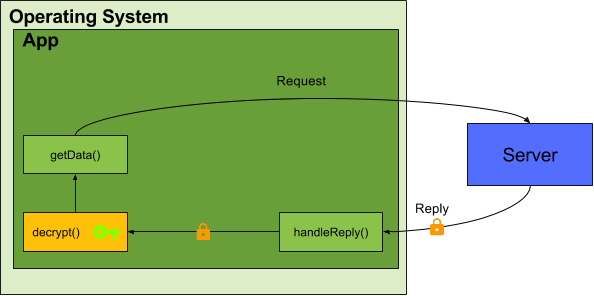
\includegraphics[width=0.8\textwidth]{data/encryptionComm.png}
    \caption{Encrypted communication with a server}
    \label{fig:encryptionComm}
\end{figure}

A similar approach is used for streaming \gls{drm} protected content on Android.
The encrypted content can only be decrypted by a native interface provided by the \gls{os} which stores the decryption key. \cite{androidDrm}
\newline
This methodology focuses on the security of the content instead of the application itself.
